\documentclass[a4paper]{book}

%PACKAGES
\usepackage[T1]{fontenc}
\usepackage[utf8]{inputenc}
\usepackage[italian]{babel}
\usepackage{amsfonts} 
\usepackage{amssymb} 
\usepackage{amsmath}
\usepackage{amsthm}		%teoremi
\usepackage{graphicx}	%immagini
\usepackage{setspace}	%interlinea
\usepackage{tikz}		%disegnare immagini
\onehalfspacing


%THEOREMS, ...
\theoremstyle{definition}
\newtheorem{ex}{Esempio}
\newtheorem{defn}{Definizione}

\theoremstyle{remark}
\newtheorem{oss}{Osservazione}
\newtheorem{dimst}{Dimostrazione}
\newtheorem{idea}{Idea}

\theoremstyle{definition}
\newtheorem{lem}{Lemma}
\newtheorem{teo}{Teorema}


%NEW COMMANDS
\newcommand{\bbx}{\mathbb{X}}
\newcommand{\bbr}{\mathbb{R}}
\newcommand{\ra}{\Rightarrow}
\newcommand{\vp}{\varphi}

\title{Calcolo delle variazioni \\ \small{Lezioni di Gobbino 17/18} }
\author{}

\begin{document}

\maketitle
\chapter{Lezione 1}
Il calcolo delle variazioni consiste nello studio di problemi di minimo.
\\
In particolar modo, abbiamo un insieme $\bbx$ ed una funzione $f:\bbx \to \bbr$ e vogliamo trovare min$\{f(x)|x \in \bbx\}$.
\\
Ci sono 4 metodi di approccio al problema:
\\
1.\textbf{Metodo indiretto}	\hspace{3mm}2.\textbf{Metodo diretto} \\
3.\textbf{Rilassamento}	\hspace{3mm}	4.\textbf{Gamma-convergenza}

\begin{ex}
\[
	f:\bbr \to \bbr, f = x^2 - 4x
\]
\[
	\textsf{Metodo indiretto: }f'(x) = 2x - 4 \ra f'(x) = 0 \iff x = 2 \ra \textit{min} = f(2) = -4
\]
Proviamo adesso a dimostrare che $f(x)$ è sempre $\leq$ di $-4$ \footnote{Questa è la vera dimostrazione}.
\[
	x^2 - 4x \ge -4 \iff x^2 -4x + 4 \ge 0 \iff (x -2)^2 \ge 0 
\]
che è vero, inoltre vale l'uguaglianza se e solo se $x = 2$. \\
Metodo diretto: dimostriamo che il minimo esiste, ad esempio usando il teorema di Weierstrass generalizzato:
\[
	f: \bbr \to \bbr \textit{ continua e } \lim_{x \to \pm\infty}f(x) = \infty \ra \textit{il minimo esiste}
\]
Ora che so che esiste posso vedere dove $f'(x) = 0$.
\end{ex}

\begin{ex}
	Cerchiamo min$\{(x^2 - 2)^2 | x \in \mathbb{Q} \}$ \\
	In questo caso il minimo non esiste. Possiamo perciò chiederci: chi è l'inf? Come sono fatte le successioni "minimizzanti"?\\
	L'inf è 0 e le succ. min. hanno una sottosuccessione che tende a $\pm \sqrt 2$.
\end{ex}
\noindent
\textbf{Rilassamento}: Con questo metodo rilassiamo le condizioni imposte dal problema e per farlo possiamo procedere in due modi:
1.Estendo f ad un ambiente più vasto; \\
2.Cambio la funzione in modo che il minimo abbia più probabilità di esistere.	

\begin{ex}
Consideriamo una famiglia di problemi di minimo:
\[
	m_n := min\{e^{x^2} + atg(x) + nsin^2(x)|x \in \bbr^n \}
\]
e chiediamoci:\\
a cosa tende $m_n$ quando $n \to\infty$?\\
a cosa tendono i punti di minimo quando $n \to\infty$?\\
Ci aspettiamo che $m_n \to m_{\infty} := min\{e^{x^2} + atg(x) | x = k\pi, k \in \mathbb{Z} \}$\\
Per rispondere a queste domande usiamo la gamma convergenza.
\end{ex}

\begin{defn}
Generalemente $\bbx$ sarà uno spazio di funzioni. Chiameremo allora 
\[
 	F :\bbx \to \bbr 
 \] 
\textbf{Funzionale}
\end{defn}

\begin{ex}
\[
	F(u) = \int_2^4 (\dot u^2 + sin(u))\,dx
\]
\end{ex}
\noindent
Un particolare tipo di funzionali sono poi quelli $\textbf{integrali}$
\[
	F(u) := \int_a^b L(x, u(x), \dot u(x))\,dx
\]
con $L: [a,b]\times\bbr\times\bbr \to \bbr$.\\
In generale scriveremo $L(x, s, p)$ dette Lagrangiane.\\
Altre generalizzazioni possibili sono:
\[
	F(u) := \int_{a}^{b} L(x, u, \dot u, \ddot u, \dots)dx
\]
\[
	F(u, v) := \int_a^b L(x, u, v, \dot u, \dot v, \dots)dx
\]

\begin{oss}
Problemi più complicati sono del tipo:\\
1.Più variabili in partenza\\
2.Più variabili in partenza e arrivo (caso vettoriale)
\end{oss}

\begin{ex}[Classico]
Data f(x) trovare\\
\[
	min\{\int_a^b \dot u^2 + (u - f)^2\,dx | u \in C^1([a,b])\}
\]

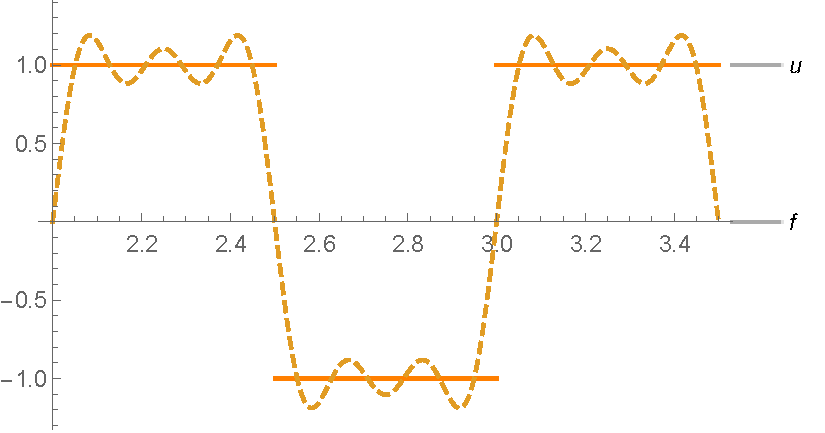
\includegraphics[scale = 0.5]{Fourier_onda_quadra.pdf}\\
\noindent
con f che può essere ad esempio il segnale di un cellulare.
\end{ex}

\begin{ex}[Classico]
\[
	min\{\int_a^b(\dot u^2 + u)dx | u(a) = A, u(b) = B, u \in C^1([a,b])\}
\]
con A e B dati\\
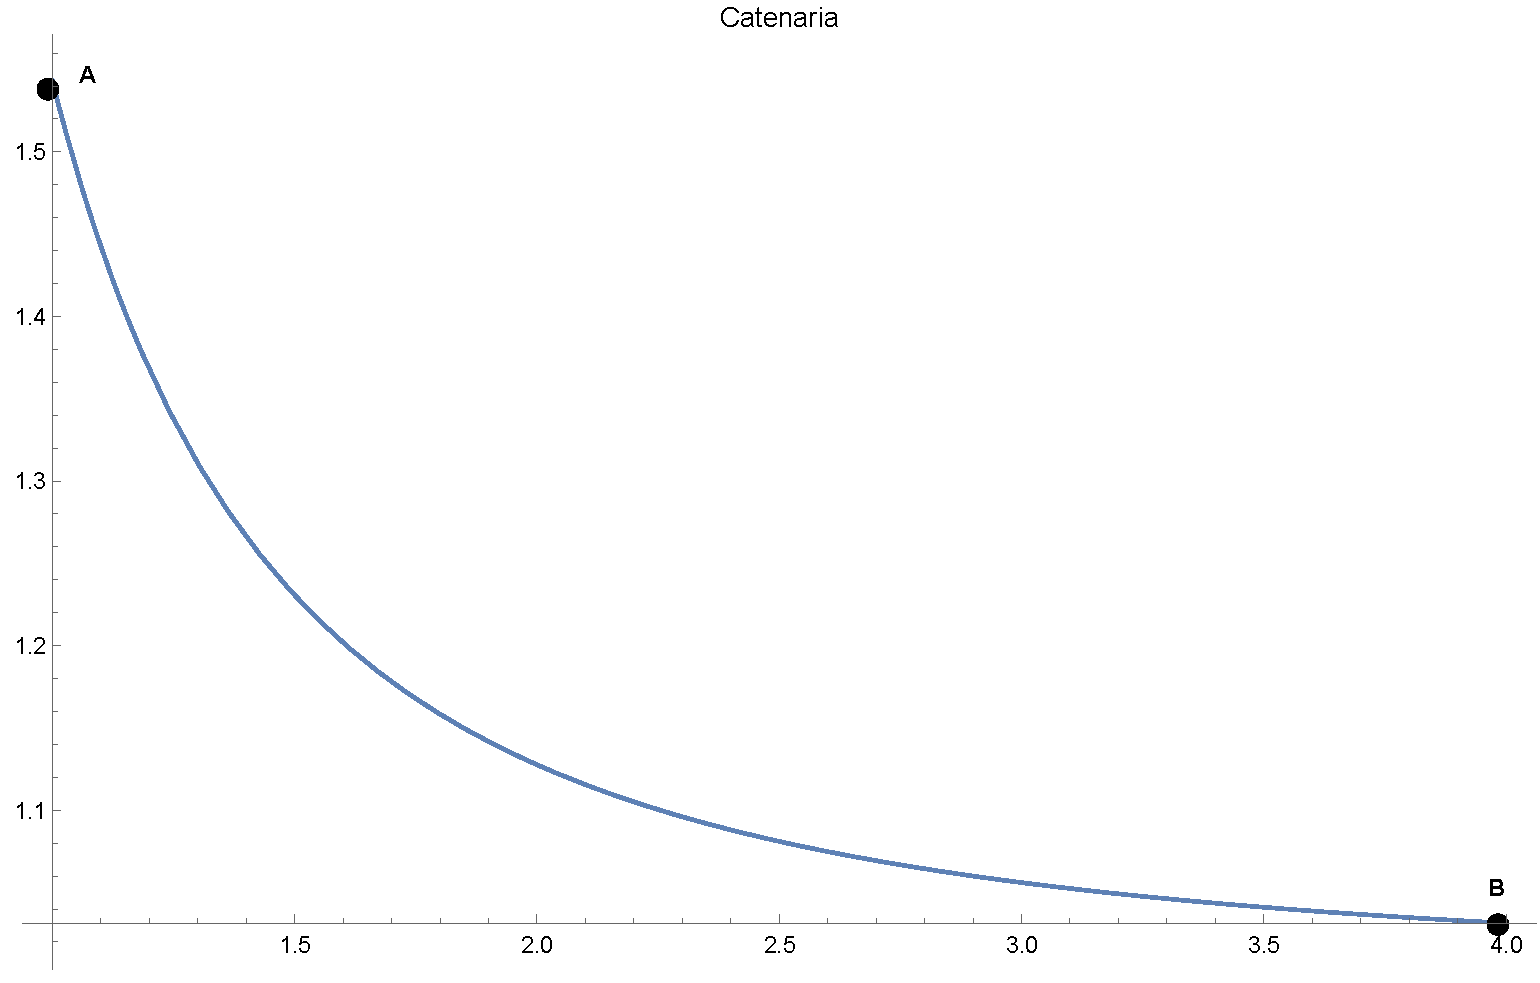
\includegraphics[scale = 0.4]{catenaria.pdf}
\end{ex}

\chapter{Lezione 2}
La variazione prima di un funzionale è l'analogo della derivata prima per una funzione.
\begin{defn}
Consideriamo un insieme $\bbx$ ed $f:\bbx \to \bbr$. Sia $x_0$ un punto di minimo e siano $\delta > 0, \gamma:(-\delta, \delta)\to \bbx$ t.c. $\gamma(0)=x_0$.
Posso considerare la funzione composta
\[
	\varphi(t) := F(\gamma(t)) \in \bbr
\]
Allora
\[
	\varphi:(-\delta, \delta)\to\bbr
\]
con minimo in t=0.\\
Pongo allora $\delta F(x_0, \gamma):=\varphi'(0)$(\footnote{Posto che esista}).\\
$\delta F(x_0, \gamma)$ è detto \textbf{Variazione prima del funzionale F lungo una curva $\gamma$}.
\end{defn}

\begin{oss}
La definizione è valida $\forall x_0$, anche non di minimo, e $\forall$ curva $\gamma : \gamma(0) = x_0$ purchè $\varphi'(0)$ esista.
\end{oss}

\begin{lem}
Se $x_0 \in argmin\footnote{$x \in \bbx$ t.c. f(x) è un minimo} \{f(x)|x\in\bbx \}$, allora 
\[
	\delta F(x_0, \gamma) = 0
\]
quando esiste.
\end{lem}
\noindent 
Supponiamo ora che $\bbx$ sia uno spazio affine con spazio vettoriale di riferimento\footnote{traslato che passa per l'origine, detto anche giacitura} V.\\
In particolare
\[
	\forall u \in \bbx, \forall v \in V \textit{ si ha che } u + v \in \bbx
\]
In questo caso, dati $u_0 \in \bbx$ e $v \in V \smallsetminus \{ 0 \}$ posso considerare la curva
\[
	t \to u_0 + tv : \textit{retta per $u_0$ con direzione v}
\]
e calcolare
\[
	\delta F(u_0, v) := \footnote{"derivata direzionale" o "alla Gateaux"} \lim_{t \to 0} \frac{F(u_0 + tv) - F(u_0)}{t}
\]

\begin{ex}
Consideriamo 3 funzionali
\[
	F(u) = \int_a^b \dot u^2(x)dx \qquad G(u) = \int_a^b |\dot u(x)|dx \qquad H(u) = \int_a^b \sqrt{|\dot u(x)|}dx
\]
con $\bbx = \{u\in C^1([a,b]) | u(a) = A, u(b) = B \}$ 


\begin{oss}
$\bbx$ è uno spazio affine con giacitura
\[
	V = \{v \in C^1([a,b])| v(a) = v(b) = 0\}
\]
\end{oss}
\noindent 
\textit{Metodo indiretto:}
\[
	\varphi(t) = F (u + tv) = \int_a^b(\dot u + t \dot v)^2\,dx = \int_a^b \dot u^2 + \int_a^b 2t\dot u \dot v + \int_a^b t^2 \dot v^2
\]
\[
	\ra \delta F(u, v) := \varphi'(0) \stackrel{\footnote{Deriviamo rispetto a t}}{=}  2\int_a^b \dot u \dot v 
\]
Questa è detta \textbf{Prima forma integrale della variazione prima}.\\
Integriamo adesso per parti:
\[
	\varphi'(0) = 2[\dot u v]_a^b - 2 \int_a^b \ddot u v = \underbrace{2(u(b)v(b)-u(a)v(a))}_{0} - 2\int_a^b \ddot u v = -2\int_a^b \ddot u v
\]
Questa, invece, è detta \textbf{Seconda forma integrale della variazione prima}.

\begin{oss}
Abbiamo usato $\ddot u$ che non è detto esista, ma tanto siamo ancora nella parte preliminare e non devo necessariamente essere formale.
\end{oss}
Allora se $u_0$ è un punto di minimo 
\[
	\int_a^b \dot u_0 \dot v = 0 \qquad \forall v \in V
\]
e se u fosse $C^2$
\[
	\int_a^b \ddot u_0 v = 0 \qquad \forall v \in V
\]
Dalla seconda sembra ragionevole dedurre che 
\[
	\ddot u_0(x) \equiv 0 \ra u_0(x) =\textit{retta } A \to B
\]
Forniamo adesso la dimostrazione rigorosa:\\
Sia $u_0(x)$ la retta e sia $w(x)$ un qualunque altro elemento di $\bbx$. Allora 
\[
	v = w - u_0 \in V
\]
quindi si annulla in a e b.
\[
	F(w) = F(u_0 + v) = \int_a^b (\dot u_0 + \dot v)^2 = \underbrace{\int_a^b \dot u_0^2}_{F(u_0)} + \underbrace{2\int_a^b \dot u_0 \dot v}_{0 \footnote{Integrando per parti poichè $u \in C^2$}} + \underbrace{\int_a^b \dot v ^2}_{\ge 0} \ge F(u_0) \qquad w(x)
\]
Abbiamo così dimostrato che $F(w) \ge F(u_0)$ e vale l'uguale $\iff \int_a^b \dot v^2 = 0\iff\dot v(x) = 0 \iff v(x) = c.te$, ma $v(a)=v(b)=0 \ra v(x)=0 \ra w(x) ) u_0(x)$.\\
Quindi la retta è l'unico punto di minimo 
\[
	\ddot u_0(x) = 0 \qquad \forall x \in [a,b]
\]
Quest'ultima equazione è detta \textbf{Forma differenziale di ELE} \footnote{Equazioni di Eulero-Lagrange}.\\

Passiamo adesso al funzionale H.\\
Dico che $infH = 0$ e non è minimo a meno del caso banale A = B.\\
Infatti
\[
	H(u_n)=\int_{b-1/n}^b |\dot u_n(x)|^2\,dx = \int_{b-1/n}^b |(B-A)n|^{1/2}\,dx = |B-A|^{1/2}\sqrt n \frac1n \to 0 \qquad \textit{per } n \to \infty
\]	
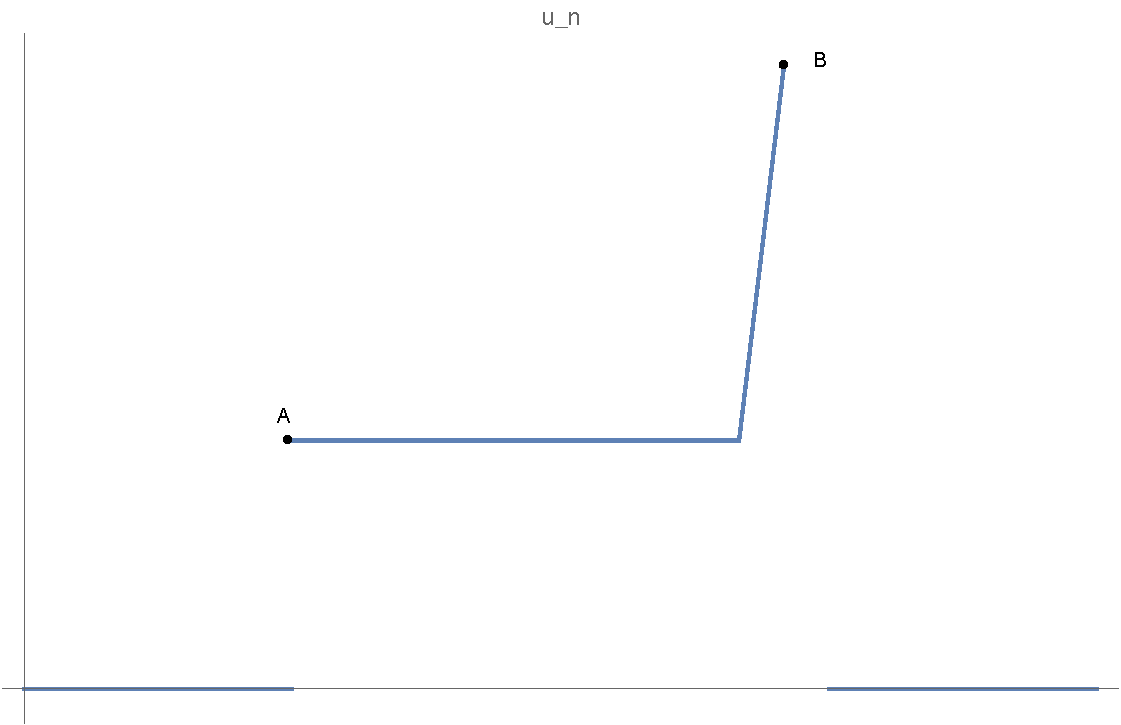
\includegraphics[scale=0.4]{u-n.pdf}

\begin{oss}
Non sarebbe $C^1$, ma fare un piccolo raccordo derivabile conta davvero poco.
\end{oss}

\begin{oss}
Fare l'$inf$ in $C^1, C^{27}, C^\infty$ o $C^1$ a tratti è sempre la stessa cosa, a patto che la Lagrangiana sia continua.
\end{oss}

Con il funzionale $G(u)$ abbiamo che il minimo esiste e i punti di minimo sono tutte le monotone.\\
Supponiamo WLOG B>A. Allora 
\[
	\int_a^b |\dot u(x)|\,dx \ge |\int_a^b \dot u(x)\,dx| = u(b) - u(a) = B-A \qquad \forall u
\]
L'uguaglianza vale se e solo se $\dot u$ ha segno costante.
\end{ex}

\begin{oss}
Lagrangiana:
\begin{itemize}
\item{Strettamente convessa in p $\to$ BUONO}
\item{Non convessa $\to$ GUAI IN VISTA}
\item{Convessa, ma non strettamente $\to$ RISCHI UNICITA' E REGOLARITA'}
\end{itemize}
\end{oss}

\chapter{Lezione 3}
\begin{lem}[Fondamentale del calcolo delle variazioni (FLCV)]
Sia $f: [a,b] \to \bbr$ continua.\\
Supponiamo che 
\[
	\int_a^b f(x)v(x)\,dx = 0 \qquad \forall v \in C^\infty_c ([a,b])	
\]
Allora 
\[
	f(x) \equiv 0 \quad \textit{in } [a,b]
\]
\end{lem}

\begin{defn}[Funzioni a supporto compatto]
$C^\infty_c ([a,b])$ implica che $\exists [c,d] \subset (a,b)$ t.c. $v(x) = 0$ fuori da $[c,d]$ (supporto compatto)
\end{defn}
Vediamo due dimostrazioni per questo teorema
\begin{dimst}[Per assurdo]
Supponiamo f non identicamente nulla, allora WLOG $\exists x_0 \in (a,b)$ t.c. $f(x_0) > 0~$(altrimenti prendo -f).\\
Allora per continuità $\exists \delta > 0$ t.c. $f(x) \ge \frac12 f(x_0) \forall x \in B(x_0, \delta$.\\
Prendo ora $v \in C^\infty (\bbr)$ t.c. 
\[
v(x) = \footnote{La $C^\infty$-tizzo} 
\begin{cases}
v(x) = 1 & x \in B(x_0, \delta) \\
v(x) = 0 & \text{altrove}
\end{cases}
\]
Allora 
\[
	\int_a^b f(x)v(x)\,dx = \int_{x_0 - \delta}^{x_0 + \delta} f(x)v(x)\,dx > 0
\]
ASSURDO \qed
\end{dimst}

\begin{dimst}[Per approssimazione]
\begin{idea}
Se
\[ 
\int_a^b f(x)v(x) = 0 \quad \forall v \in C^\infty_c \ra \int_a^b f(x)v(x)=0 \quad v\in C^0
\]
\end{idea}	
Supponendo vero questo, prendiamo 
\[
	v(x) \equiv f(x) \ra \int_a^b f^2(x) = 0 \iff\footnote{Integriamo una funzione sempre positiva} f(x)=0
\]
Fatto di approssimazione: $\forall v:[a,b] \to \bbr$ continua, esiste una successione di funzioni $\{v_n\} \subseteq C^\infty_c((a,b))$ t.c.\\
1. $\exists M$ t.c. $|v_n(x)| \le M \quad \forall n \in \mathbb{N} \quad\forall x \in [a,b] $ (poichè v continua)\\
2. $v_n(x) \stackrel{u}{\to} v(x)$ sui compatti $K \subset (a,b)$\\
Questo basta per concludere che 
\[
	\lim_{n \to \infty}\int_a^b v_n(x)f(x)\,dx = \int_a^b v(x)f(x)\,dx
\]
\textit{Fisso $\epsilon > 0$ e ho convergenza degli integrali in $[a+\epsilon, b- \epsilon]$. Gli integrali in $[a, a+\epsilon],[b- \epsilon, b]$ si stimano per equilimitatezza.}
\end{dimst}

\begin{oss}[Generalizzazioni]
Possiamo adesso chiederci per quali classi di funzioni V vale il lemma?\\
1. Se l'integrale è nullo $\forall v \in V$, allora è nullo $\forall v \in Span\{v\}$.\\
2. Se l'integrale è nullo $\forall v \in V$, allora è nullo sulla chiusura di V rispetto alla convergenza uniforme sui compatti contenuti in $[a,b] \smallsetminus \{\text{numero finito di punti}\} $. (si dimostra per approssimazione).
\end{oss}

Il lemma allora funziona per tutti gli spazi t.c. $\overline{Span\{v\}} = C^0 $.

\begin{lem}[Du Bois-Reymond (DBR)]
Sia $f:[a,b]\to\bbr $ continua. Supponiamo che 
\[
	\int_a^b f(x)v(x)\,dx = 0\quad \forall v \in C^\infty_c((a, b)) \text{ t.c. } \int_a^b v(x)\,dx = 0
\]
Allora
\[
	f(x) \equiv \text{ c.te } \quad \text{ in } [a,b]
\]
\end{lem}

\begin{dimst}[Per assurdo]
\begin{idea}
Se f soddisfa l'ipotesi allora anche $f(x) + c$ la verifica $\forall c \in \bbr$
\end{idea}
Sia f non costante, allora WLOG $\exists x_0,y_0 $ t.c. $f(x_0) < f(y_0)$.\\
A meno di aggiungere una costante, posso assumere $f(x_0) = -f(y_0)$.\\
Considero allora v del tipo\\ 
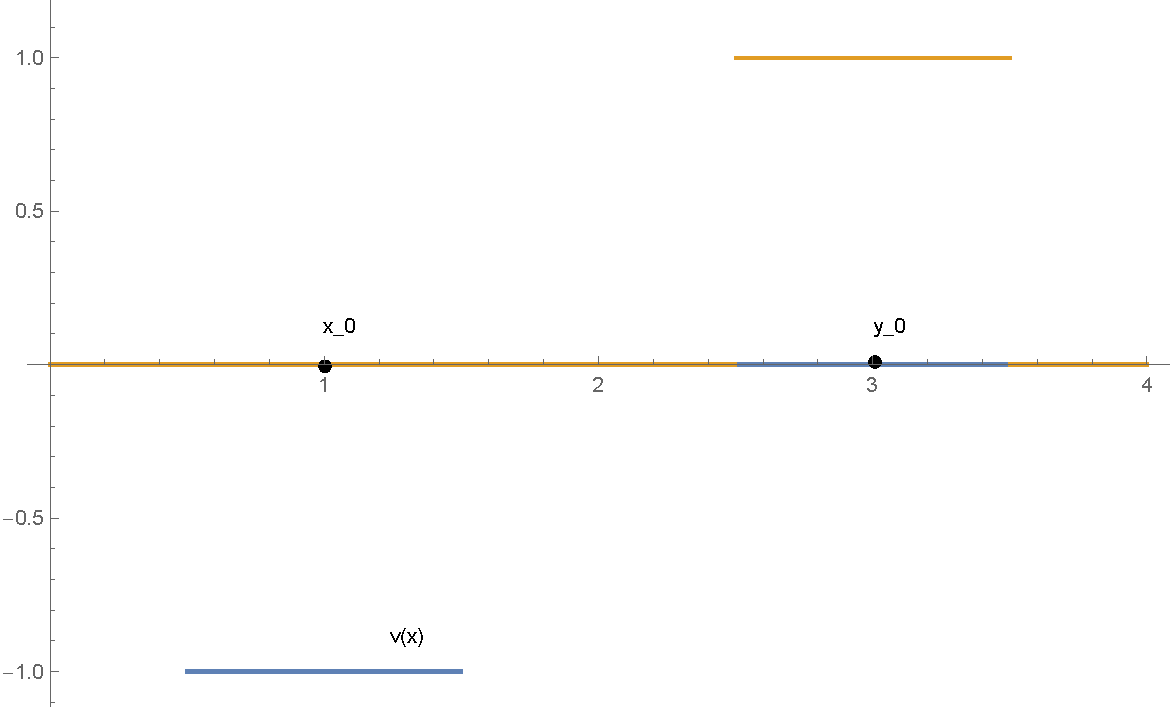
\includegraphics[scale=0.4]{dbr.pdf}
dove v è simmetrica.\\
Allora
\[
	\int_a^b f(x)v(x)\,dx > 0
\]
ASSURDO \qed
\end{dimst}

\begin{dimst}[Per approssimazione]
Si dimostra che ogni funzione $v \in C^0$ a media nulla si può approssimare con funzioni $v \in C^\infty_c((a,b))$ a media nulla e quindi 
\[
	\int_a^b f(x)v(x)\,dx = 0\quad \forall v \in C^\infty_c \text{ con } \int_a^b v(x) = 0 
\]
\[
	\ra \int_a^b f(x)v(x)\,dx = 0 \quad \forall v \in C^0 \text{ con } \int_a^b v(x)\,dx = 0
\]
A questo punto prendo $c \in \bbr $ t.c. $\int_a^b (f(x)+c)\,dx = 0$ e uso $v(x) = f(x)+c$. Ottengo quindi che $f(x) + c \equiv 0 \ra f(x)$ è costante. \qed
\end{dimst}
Anche in questo caso posso usare classi più ristrette di funzioni.\\
\begin{ex}
\[
	min\{\int_0^2 \dot u^2\,dx |\underbrace{ u(0) = 0, u(2) = 5, \int_0^2 u(x)\,dx = 7}_{\bbx}\}
\]
Osserviamo che $\bbx$ è uno spazio affine con giacitura
\[
	V := \{v \in C^1([0,2])|v(0) = 0, v(2) = 0, \int_0^2v(x)\, dx = 0 \}
\]
Data $u \in \bbx$ e $v \in V$ calcolo
\[
	F(u + tv) = F(u) + 2t \int_0^2 \dot u \dot v + t^2\int_0^2\dot v^2
	\ra \delta F(u,v) = \lim_{t\to0} \frac{F(u+tv)-F(u)}t = 2\int_0^2\dot u \dot v
\]
Integrando per parti e supponendo $u \in C^2$ troviamo
\[
	\delta F (u,v) = -2 \int_0^2 \ddot u v
\]
Quindi se u è un punto di minimo deve verificare
\[
	\int_0^2 \ddot u v = 0
\]
\[
	\forall v \in C^1([0,2]) \text{ t.c. } \int_0^2v(x) = 0, v(0)=v(2)=0
\]
Possiamo allora applicare il lemma DBR e quindi $\ddot u = $ costante $\ra u(x) = ax^2+bx+c$.\\
Imponendo le 3 condizioni trovo poi a,b,c.\\
Una volta trovato il punto di minimo faccio la dimostrazione con la disuguaglianza.
\end{ex}
\begin{lem}[DBR altro enunciato]
\[
	\int_a^b f(x)\dot v(x)\, dx = 0\quad \forall v \in C^\infty_c((a,b))
\]
Allora
\[
	f(x) \equiv \text{ c.te in } [a,b]
\]
\end{lem}

\begin{dimst}
Basta osservare che le funzioni $\dot v$ con $v \in C^\infty_c((a,b))$ sono tutte e sole le $w \in C^\infty_c$ a media nulla (l'integrale è ka differenza tra i valori agli estremi).
\end{dimst}

\begin{ex}
\begin{enumerate}
\item{$\int_a^b fv = 0\quad \forall v \in C^\infty_c \text{ t.c. } \int_a^b v = 2017 $}
\item{$\int_a^b f \ddot v = 0\quad v \in C^\infty_c $}
\end{enumerate}
\begin{enumerate}
\item{$f = 0$, la dimostrazione è analoga a quella per v a media nulla}
\item{$f(x)$ è una funzione affine del tipo $ax + b$}
\end{enumerate}
\end{ex}

\begin{oss}
Stiamo con questi lemmi cercando l'ortogonale in $L^2([a,b]) $ di un certo sottoinsieme V.
\end{oss}

\chapter{Lezione 4}
In questo capitolo studiamo la nascita delle condizioni al bordo (BC).\\

\begin{ex}
\[
	F(u)= \int_0^1 \dot{u}^2 + u^2\, dx
\]
\[
	\bbx = \{u \in C^1([0,1]) | u(0) = A, u(1) = B \}	
\]
\[
	F(u + tv) = \int_0^1 (\dot{u} + t \dot{v})^2 + (u + tv) = \int_0^1 (\dot{u}^2 + 2t \dot{u} \dot{v} +t^2 \dot{v}^2 + u^2 +2tuv + t^2v^2)
\]
\[
	\ra \delta F(u, v) = 2 \int (\dot{u} \dot{v} +uv) \qquad{\textbf{1° forma integrale}}
\]
Integrando, poi, per parti otteniamo 
\[
	\delta F(u, v) = 2 \int_{0}^{1}(-\ddot{u}v+uv) = 2 \int_{0}^{1}(-\ddot{u}+u)v \qquad{\textbf{2° forma integrale}}
\]
\begin{oss}
Ricordiamo che i termini di bordo sono nulli poichè $v(0)=v(1)=0$
\end{oss}
\noindent 
Se u è un punto di minimo, allora per FLCV
\[
	-\ddot{u} + u \equiv 0 \ra \underbrace{\ddot{u} = u}_{ELE}, \underbrace{u(0) = A, u(1) = B}_{\text{DBC, Dirichlet Boundary Condition}}	
\]
\end{ex}

\begin{ex}
Consideriamo la stessa $F(u)$, ma adesso $\bbx = \{u \in C^1([0,1])|u(0) = A \} $\\
In questo caso $V = \{v \in C^1([0,1])|v(0) = 0 \} $\\
Allora 
\[
	\delta F(u,v) = 2 \int_{0}^{1} \dot{u} \dot{v} + uv
\]
Integrando per parti allora otteniamo 
\begin{align}
	\delta F(u,v) &=  2 \int_{0}^{1} (-\ddot{u}v + uv) + [\dot{u}	v]_0^1 \\
	& = 2 \int_{0}^{1}(-\ddot{u} +u)v + u(1)v(1)
\end{align}
In questo caso la seconda forma integrale contiene un termine di bordo.\\
Se u è un punto di minimo, allora questa è 0 $\forall v \in V$.\
Procedo in due fasi:\\
1. Mi limito a considerare le v che verificano anche $v(1) = 0$. Ottengo quindi la stessa equazione del primo esempio $\ddot{u}	= u $.\\
2. Adesso l'equazione diventa 
\[
	\dot{u}(1) \dot{v}(1) = 0
\]
allora basta prendere $v \in V$ con $v(1) \not = 0 $ per ottenere che $\dot{u}(1) = 0$\\
Alla fine si ottiene
\[
\begin{cases}
	\ddot{u} = u, & ELE \\
	u(0) = A, & DBC \\
	\dot{u}(1) = 0, & NBC, \text{ Neumann boundary condition}
\end{cases}
\]
Si conclude poi sempre mediante disuguaglianza.
\end{ex}

\begin{ex}
Stessa $F(u)$, $\bbx = \{ u \in C^1([0,1])\}$. Nascono in questo caso le due Neumann agli estremi:
\[
	\begin{cases}
	\ddot{u} = u\\
	\dot{u}(0) = 0\\
	\dot{u}(1) = 0
	\end{cases}
\]
\end{ex}	

\begin{ex}
$\bbx = \{u \in C^1([0,1])| u(0) = u(1)$. In questo caso $\bbx$ è uno spazio vettoriale quindi $V = \bbx$.
\begin{align}
\delta F(u,v) &= 2 \int_{0}^{1}(-\ddot{u}+u)v + 2\dot{u}(1)v(1) - 2\dot{u}(0)v(0)\\
& = 2 \int_{0}^{1}(-\ddot{u}+u)v + 2v(0)(\dot{u}(1) - \dot{u}(0))
\end{align}
Nella prima fase pongo $\ddot{u} = u$, mentre nella seconda prendo v con $v(0)=v(1)\not=0$ ed ottengo $\dot{u}(1)=\dot{u}(0)$.
Devo allora risolvere
\[
	\begin{cases}
	\ddot{u} = u\\
	\dot{u}(0) = \dot{u}(1)\\
	u(0) = u(1)
	\end{cases}
\]
Le ultime due condizioni sono dette \textbf{PBC, Periodic BC}
\end{ex}

\begin{ex}
$\bbx =\{u \in C^1([0,1])| u(0) = u(1) + 5\} \ra V =\{v \in C^1([0,1])| v(0) = v(1)\} $\\
Con lo stesso conto di prima troviamo che $\dot{u}(1) = \dot{u}(0)$ e quindi 
\[
	\begin{cases}
	\ddot{u} = u\\
	\dot{u}(0) = \dot{u}(1)\\
	u(0) = u(1) + 5
	\end{cases}
\]
\end{ex}

\begin{ex}
$\bbx =\{u \in C^1([0,1])| u(\frac12) = A\} \ra V =\{v \in C^1([0,1])| v(\frac12) = 0\} $\\
Quindi
\[
	\frac12 \delta F(u, v) = \int_{0}^{1}(-\ddot{u} + u)v + \dot{u}(1)v(1) - \dot{u}(0)v(0)
\]
Nella prima fase uso v con $v(0)=v(1)=0$ oltre a $v(\frac12)=0$. Allora per FLCV $\ddot{u} = u$.\\
Dalla seconda fase ottengo poi, come NBC, $\dot{u}(1)=\dot{u}(0)=0$.Ottengo quindi
\[
	\begin{cases}
	\ddot{u} = u\\
	\dot{u}(0) = \dot{u}(1) = 0\\
	u(\frac12) = A
	\end{cases}
\]
che sono in generale troppe condizioni.\\
Si verificano quindi due casi:\\
1. C'è la soluzione e con la disuguaglianza posso mostrare che è un minimo;\\
2. Le condizioni sono incompatibili e quindi il minimo non esiste. Ci possiamo quindi chiedere chi sia l'inf.\\
Per rispondere a questa domanda risolvo i problemi separatamente

\[
	\begin{cases}
	\ddot{u} = u\\
	\dot{u}(0) = 0\\
	u(\frac12) = A
	\end{cases}
\]

\[
	\begin{cases}
	\ddot{u} = u\\
	\dot{u}(1) = 0\\
	u(\frac12) = A
	\end{cases}
\]
Accade dunque che in $\frac12$ non si incollano $C^1$.
\end{ex}

\begin{oss}
Se fosse stato $F(u) = \int \ddot{u}^2+ u^2$, allora ELE di ordine 4, cioè il grado di ELE è sempre il doppio dell'ordine di derivazione.
\end{oss}

\begin{oss}
Se nel problema iniziale metto $\dot{u}(0) = 3$ ottengo come sempre che $\ddot{u} = u$ e che 
\[
	\dot{u}(1) v(1) - \dot{u}(0)v(0) = 0 \ra \dot{u}(1) = \dot{u}(0) = 3
\]
quindi non esiste il minimo, ma più in generale se $F(u)$ dipende da u e $\dot{u}$ non posso mettere condizioni su $\dot{u}$.
\end{oss}

\chapter{Lezione 5}
\section{Equazione di Eulero-Lagrange}

Sia
\[
	F(u) = \int_{a}^{b}L(x, \dot{u}, \ddot{u})\, dx
\]
con 
\[
	L : \underbrace{[a,b]}_{\ni x}\times \underbrace{\bbr}_{\ni s}\times\underbrace{\bbr}_{\ni p} \to \bbr
\]
Data $u: [a,b] \to \bbr$ e data $v: [a,b] \to \bbr$ con $v(a)=v(b)=0$ posso definire
\[
	\psi(t) := F(u+tv) = \int_{a}^{b}L(x, u+tv, \dot{u} + t \dot{v})\, dx
\]
e porre 
\[
	\delta F(u,v) := \psi'(0)
\]

\begin{teo}[Integrali dipendenti da parametro]
Sia $[a,b] \subseteq \bbr$ un intervallo, sia $\delta >0$, sia 
\[
	f:[a,b]\times(-\delta, \delta) \to\bbr \qquad x \in [a,b], t\in (-\delta,\delta)
\]
Poniamo 
\[
	\psi(t) := \int_{a}^{b}f(x, t)\,dx
\]
Allora
\begin{enumerate}
\item{Se $f(x,t)$ è continua in $[a,b]\times(-\delta, \delta)$, allora $\psi(t)$ è continua in $(-\delta,\delta)$;}
\item{Se $f_t(x,t)$ è continua in $[a,b]\times(-\delta,\delta)$, allora $\psi$ è derivabile e \\ $\psi '(t) = \int_{a}^{b}f_t(x,t)\,dx$. Cioè la derivata dell'integrale è l'integrale della derivata.}
\end{enumerate}
\end{teo}

Utilizzando il teorema otteniamo che
\[
	\psi '(t) = \int_{a}^{b}L_s(x, u+tv, \dot{u} + t\dot{v})v + L_p(x, u+tv, \dot{u} +t \dot{v}) \dot{v}\, dx
\]
da cui 
\[
	\delta F(u,v) = \psi'(0)=\int_{a}^{b}[L_s(x,u, \dot{u})v + L_p(x, u, \dot{u}) \dot{v}]\,dx
\]
che è quella che avevamo chiamato la \textbf{Prima forma integrale della variazione prima}.\\

\begin{oss}
Abbiamo utilizzato come ipotesi che $L \in C^1$ in s e p, $u \in C^1, v \in C^1$. Non abbiamo ancora utilizzato $v(a)=v(b)=0$, che useremo per la seconda forma.
\end{oss}

Integrando poi per parti il secondo termine troviamo 
\[
	\int_{a}^{b}L_p(x, u, \dot{u}) \dot{v}\,dx = [L_p(x, u, \dot{u})v]_a^b - \int_{a}^{b}[L_p(x, u, \dot{u})]' v\,dx
\]
Se $v(a)=v(b)=0$, il termine di bordo si annulla e troviamo
\[
	\delta F(u,v) = \int_{a}^{b}[L_s(x, u, \dot{u}) - L_p'(x, u, \dot{u})]v\,dx
\]
detta \textbf{Seconda forma integrale della variazione prima}.

\begin{oss}
Qui utilizziamo $L \in C^2, u \in C^2, v \in C^1$ e $v(a)=v(b)=0$.
\end{oss}

Se u è un punto di minimo (tra quelli che hanno lo stesso dato al bordo), allora la $\delta F(u,v) = 0 ~\forall v \in V$. Allora utilizzando il lemma fondamentale ottengo che
\[
	[L_p(x, u, \dot{u})]' = L_s(x, u, \dot{u})
\]
ELE in forma differenziale.

\begin{oss}[Condizione di Neumann in generale]
\[
	u \in argmin\{F(u) | \underbrace{u \in C^1([a,b]), u(a)=A}_{\bbx} \}
\]
Se c'è abbastanza regolarità, usando solo v con $v(a)=v(b)=0$ ritroviamo ELE come sopra.\\
Integrando per parti la prima forma troviamo
\[
	0 = \delta F(u,v) = \int_{a}^{b}\underbrace{[(L_p(x, u, \dot{u}))' - L_s(x, u, \dot{u})]}_{0 \text{ per ELE}}v\,dx + [L_p(x, u, \dot{u})v]_a^b
\]
\[
	\ra L_p(b, u(b), \dot{u}(b))v(b) - L_p(a, u(a), \dot{u}(a))v(a) = 0 
\]
adesso posso mettere $v(a)=0$, ma $v(b)$ può essere $1$, quindi si ha una condizione su $L_p$ in un estremo.
\[
	L_p(x, u, \dot{u}) = 0 \qquad \text{ nell'estremo considerato è detta NBC generale}
\]
\end{oss}

\begin{oss}
L'equazione ELE
\[
	[L_p(x, u, \dot{u})]' = L_s(x, u, \dot{u})
\]
espansa diventa
\[
	L_{px}(x, u, \dot{u}) + L_{ps}(x, u, \dot{u})\dot{u} + L_{pp}(x, u, \dot{u})\ddot{u} = L_s(x, u, \dot{u})
\]
che si può scrivere in forma normale e quindi soddisfa il teorema di Cauchy-Lipschitz se 
\[
	L_{pp}(x, u, \dot{u}) \not = 0 \qquad \forall x \in [a.b]
\]
\end{oss}

\subsection{ELE in forma DBR}
Scrivo la prima forma integrale, introduco la funzione 
\[
	\hat{L}(x) := \int_{a}^{x}L_s(t, u(t), \dot{u}(t))\,dt
\]
e osservo che 
\[
	\int_{a}^{b}L_s(x, u, \dot{u})v = [\hat{L}(x)v(x)]_a^b - \int_{a}^{b} \hat{L}(x)\dot{v}(x)\,dx
\]
Il termine di bordo si annulla e ottengo
\[
	\delta F(u, v) = \int_{a}^{b}[\hat{L}(x) + L_p(x, u, \dot{u})]\dot{v}\,dx
\]
Se u è un punto di minimo/massimo, allora dal lemma DBR otteniamo che
\[
	L_p(x, u, \dot{u}) = c + \int_{a}^{x}L_s(t, u(s), \dot{u}(s))\,ds \quad \text{ ELE-DBR}\footnote{serve meno regolarità in L ed u}
\]

\subsection{ELE in forma ERDMANN}
Consideriamo il caso in cui la Lagrangiana non dipenda da x.
\[
	(L_p(u, \dot{u}))' = L_s(u, \dot{u})
\]
Moltiplico a destra e sinistra per $\dot{u}$ ed ottengo


$$(L_p(u, \dot{u}))'\dot{u} = L_s(u, \dot{u})\dot{u} $$
$$\ra (L_p(u, \dot{u}) \dot{u})' - L_p(u, \dot{u})\ddot{u} = L_s(u, \dot{u}) \dot{u}$$
$$\ra (L_p(u, \dot{u}) \dot{u})' = L_s(u, \dot{u})\dot{u} + L_p(u, \dot{u})\ddot{u}$$
$$\ra (L_p(u, \dot{u}) \dot{u})' = (L(u, \dot{u}))'$$

e quindi
\[
	L_p(u, \dot{u}) \dot{u} = L(u, \dot{u}) + c
\]
questa è detta equazione \textbf{ELE-Erdmann}.

\begin{oss}
Questa è un'equazione differenziale di ordine 1.
\end{oss}
\begin{oss}
ELE classica ed ELE Erdmann \underline{non} sono equivalenti, ma
\[
\text{u soddisfa ELE classica} \ra \text{ u soddisfa ELE-Erdmann}		
\]	
\[
\text{u soddisfa ELE-Erdmann} \ra \text{ u soddisfa ELE classica nei punti } x\in[a,b] \text{ t.c. }  \dot{u}(x) \not= 0 \footnote{Basta fare i passaggi al contrario}
\]
\end{oss}	

\begin{oss}[Piccola generalizzazione]
Consideriamo il caso in cui F dipenda da più derivate successive
\begin{align}
	F(u) & = \int_{a}^{b}L(x, u, \dot{u}, \ddot{u}, \dots, u^{(k)})\,dx \\
	& = \int_{a}^{b}L(x, s, p_1, \dots, p_k)
\end{align}
\[
	\delta F(u, v) = \int_{a}^{b}L_s(\dots)v + L_{p_1}(\dots) \dot{v} + \dots + L_{p_k}(\dots) v^{(k)}
\]
Integrando per parti e supponendo v abbastanza nulla al bordo
\[
 	\delta F(u, v) = \int_{a}^{b}[L_s - (L_{p_1})' + (L_{p_2})''+ \dots]v\,dx
\] 
Quindi se u è un punto di min/max dal FLCV troviamo
\[
	\sum^{k}_{i=1} (-1)^{i+1}\frac{d^i}{dx^i}L_{p_i}(x, u, \dot{u}, \dots, u^{k}) = L_s(x, u, \dot{u}, u^{k})
\]
che è la ELE per dipendenza da più derivate.
\end{oss}

\chapter{Lezione 6}
\section{Come dimostrare che u è un minimo di F}
Alcune strategie possibili:\\
\begin{enumerate}
\item Convessità
\item Lemma trivial
\item Calibrazioni
\item Campi di Weierstrass
\end{enumerate}

\subsection{Convessità}
Da analisi 1 sappiamo che: se $f:[c,d]\to\bbr$ è una funzione convessa e $x_0 \in (c,d)$, allora esiste una costante $m\in\bbr$ tale che 
\[
	f(x)\ge f(x_0)+m(x-x_0)\quad\forall x \in [c,d]
\]
In generale basta prendere $m \in [f_-'(x_0), f_+'(x_0)]$.\\
Da analisi 2 sappiamo che: se $f(x,y)$ è convessa e se $(x_0, y_0)\in \bbr$, allora esistono $m_1\in\bbr, m_2\in\bbr$ t.c.
\[
	f(x, y)\ge f(x_0, y_0) + m_1(x-x_0) + m_2(y-y_0)\quad \forall(x,y)\in\text{Dominio}
\]

\begin{teo}
Consideriamo adesso $F(u) = \int_{a}^{b}L(x, u, \dot{u})\,dx$ con DBC.\\
Supponiamo che:\\
\begin{enumerate}
\item Ci sia abbastanza regolarità
\item $u_0(x)$ sia soluzione di ELE con DBC
\item $\forall x \in [a,b]$ la funzione $(s,p)\to L(x, s, p)$ è convessa come funzione di due variabili.
\end{enumerate}
Allora $u_0$ è un punto di minimo per il problema con le DBC.
\end{teo}

\begin{dimst}
Prendo un qualunque altro competitore w e pongo $v(x) := w(x)-u(x)$ ed osservo che $v(a)=v(b)=0$. Scrivo che 
\[
	F(w) = F(u_0 + v) = \int_{a}^{b} L(x, u_0 + v, \dot{u_0} + \dot{v})\,dx
\]
Dopodichè dalla convessità e regolarità di L ottengo la disuguaglianza
\[
	L(x, s +s_1, p+p_1)\ge L(x, s, p) + L_s(x, s, p)s_1 + L_p(x, s, p)p_1
\]
Prendendo poi $s = u_0 , s_1 = v, p = \dot{u}_0, p_1 = \dot{v}$ si ha che
\[
	F(w)\ge \int_{a}^{b}L(x, u_0, \dot{u}_0) + \underbrace{L_s(x, u, \dot{u}_0)v + L_p(x, u_0, \dot{u}_0)\dot{v}}_{= 0 \text{ per la prima forma integrale di ELE}}
\]
\[
	\ra F(w)\ge \int_{a}^{b}L(x, u_0, \dot{u_0}) = F(u_0) \qed
\]
\end{dimst}

\begin{oss}
Abbiamo in realtà usato solo che $u_0$ risolve la prima forma integrale di ELE, che richiede meno regolarità su L. Inoltre, se L fosse strettamente convessa in $(s, p)$, allora la disuguaglianza di analisi 2 è stretta se $(x, y) \not = (x_0, y_0)$, da cui l'unico modo per avere uguaglianza è che v e $\dot{v}$ siano nulle, cioè $v(x) \equiv 0$. Quindi $u_0$ è l'unico punto di minimo. 
\end{oss}

\begin{ex}
$$
F(u) = \int_{0}^{1} (\dot{u}(x))^4\, dx
$$
e minimizzo con $u(0) = 0, u(1) = 5$. Allora
\[
	L(x, s, p) = p^4 \ra [L_p(x, s, p)]' = L_s(x, s, p) \ra (4 \dot{u}^3)' = 0 \ra \dot{u} = c.te\ra u = \text{retta}
\]
Per l'enunciato precedente, la retta è l'unico punto di minimo; tuttavia se non pensiamo alla convessità è meno evidente:
\[
	F(w) = F(u+v) = \int_{0}^{1}(\dot{u} + \dot{v})^4 = \int_{0}^{1}(\underbrace{\dot{u}^4}_{=F(u)} + \overbrace{4\dot{u}^3 \dot{v}}^{=0 \text{ integrando per parti ed usando ELE}} + \underbrace{6 \dot{u}^2 \dot{v}^2 + 4 \dot{u} \dot{v}^3 + \dot{v}^4}_{\ge \text{ ma non del tutto evidente}\footnote{Forma quadratica definita positiva, tutttavia fare i conti non è sempre una buona idea. Questa volta ci salva l'esponente basso}})
\]
\end{ex}

\begin{lem}[Lemma trivial]
Sia $\bbx$ un insieme, e siano $F:\bbx \to\bbr$ e $G:\bbx\to\bbr$ due funzioni. Supponiamo che
\begin{enumerate}
\item $F(x) \ge G(x) \quad \forall x\in \bbx$
\item $x_0 \in \bbx$ è punto di minimo di G
\item $F(x_0) = G(x_0)$ 
\end{enumerate}
Allora $x_0$ è punto di minimo per F.
\end{lem}

\begin{dimst}
\[
	\forall x \in \bbx \text{ vale: } F(x)\underbrace{\ge}_{1}G(x)\underbrace{\ge}_{2} G(x_0)\underbrace{=}_{3}F(x_0)\qed
\]
\end{dimst}

\begin{ex}
Consideriamo il funzionale $F(u) = \int_{o}^{2}(\dot{u}^2 - 1)^2\,dx$ e l'insieme $\bbx = \{ u \in C^1([0,2])| u(0)=1, u(2)=7\}$. In questo caso la Lagrangiana non è convessa in p come si evince dalla figura$\qquad$
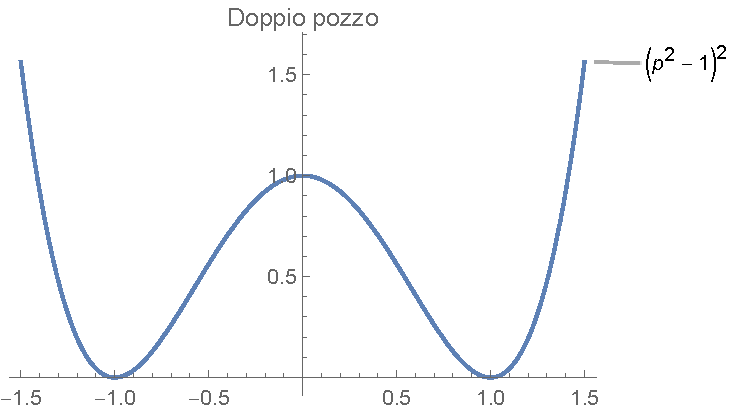
\includegraphics[scale=0.4]{doppio-pozzo.pdf}.\\
Supponiamo adesso che la retta $u_0(x) := 1 +3x$ sia l'unico punto di minimo e troviamo la G giusta.\\
\textit{Idea:} convessifico L. Considero
\[
	\hat{L}(p) = \begin{cases}
	L(p) & |p|\ge 1 \\
	0 & |p| \le 1
	\end{cases}
\]
ed osservo che $\hat{L}$ è convessa. Pongo
\[
	G(u) := \int_{0}^{2} \hat{L}(\dot{u})\,dx
\]
e verifico le ipotesi.\\
(1) segue da $L \ge \hat{L}$; (2) segue dalla convessità di $\hat{L}$, quindi $u_0$ è punto di minimo per G; (3) segue dal fatto che $L(3) = \hat{L}(3)$. Da questo segue che $u_0$ è punto di minimo per F. Inoltre G ha come unico minimo $u_0$, in quanto $\hat{L}$ strettamente convessa in un intorno di $p=3$, quindi $u_0$ è l'unico punto di minimo di G.
\end{ex}

\begin{oss}
Cosa succede nell'esempio se $\bbx = \{ u \in C^1([0,1])| u(0)=1, u(1)=2\}$?\\
In questo caso la retta $u_0(x) = 1 + \frac12 x$ non è punto di minimo, anzi il minimo non esiste e l'inf è 0.\\
\begin{figure}[h]
\centering
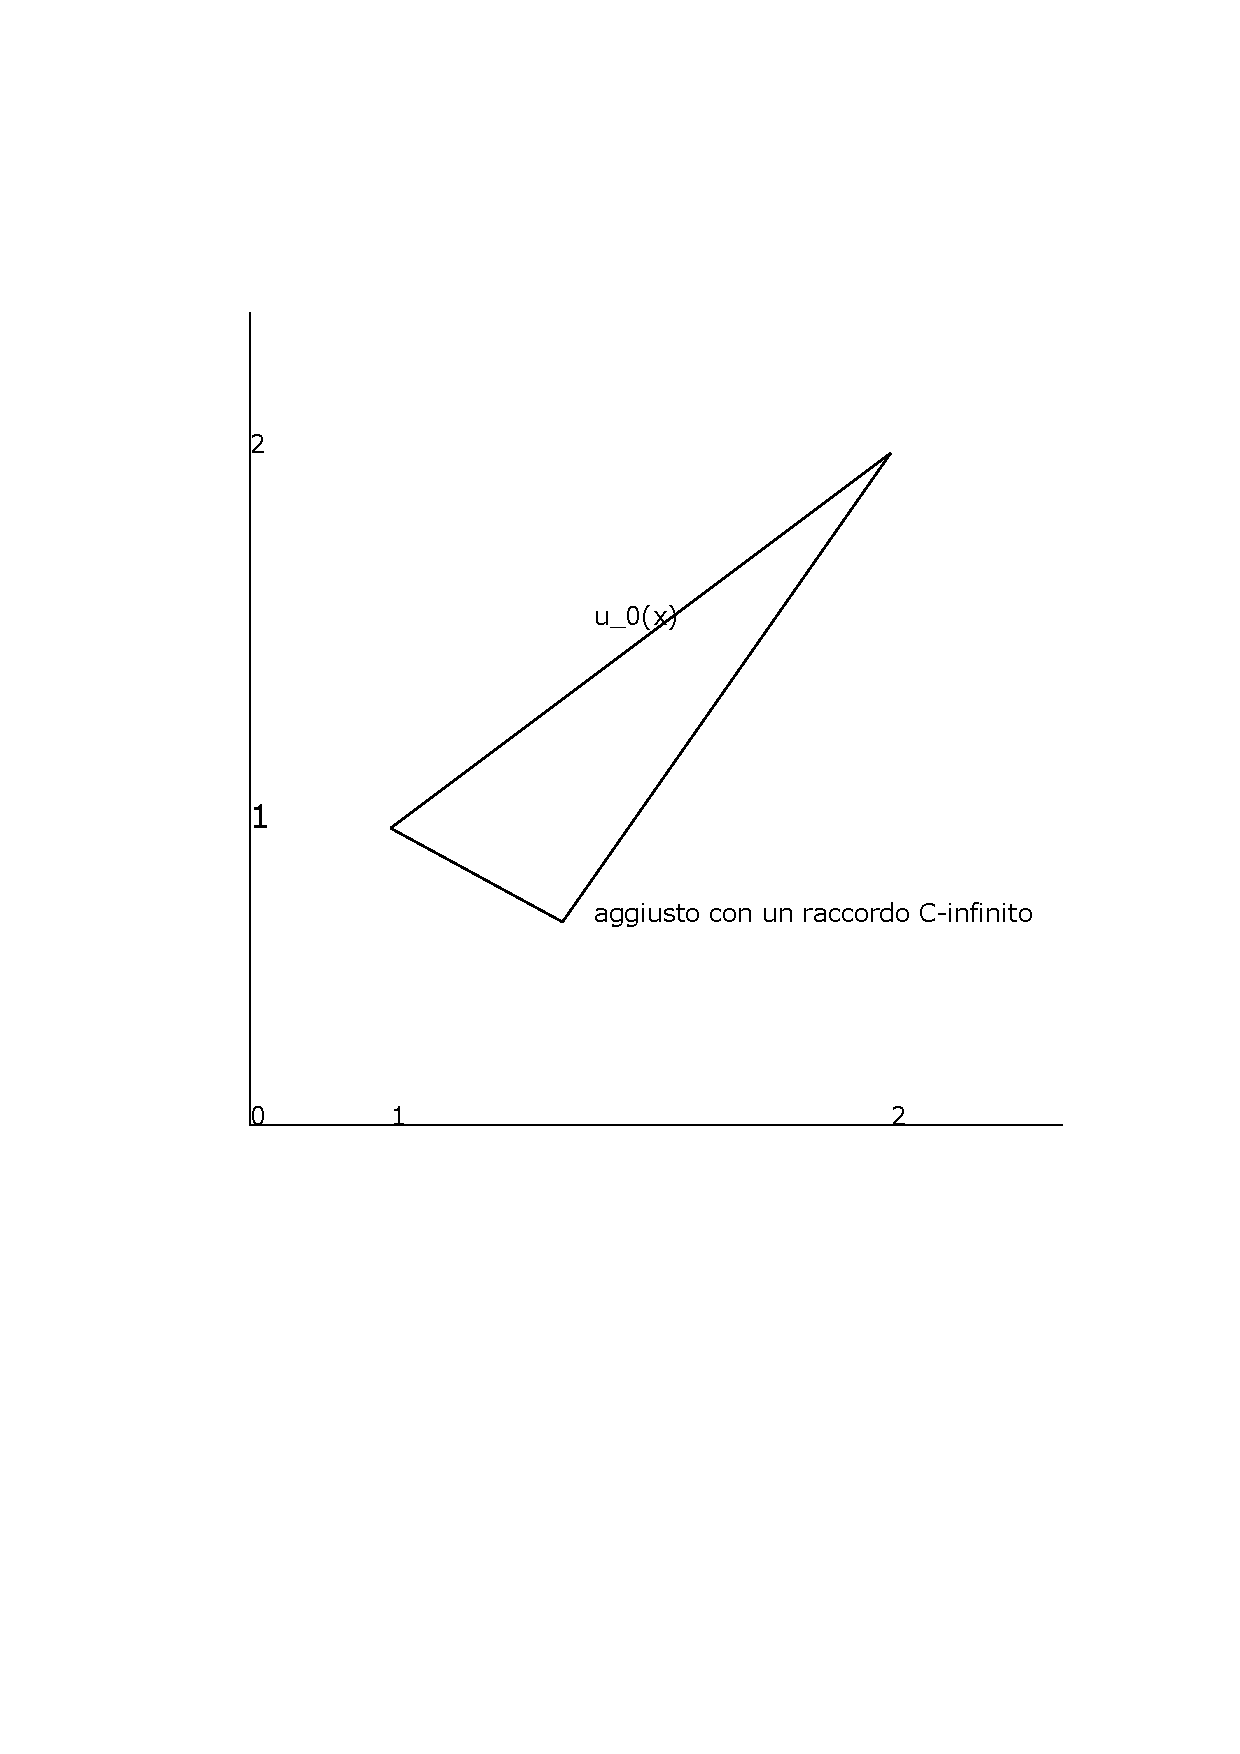
\includegraphics[scale=0.3]{capitolo6.pdf}
\end{figure}
\end{oss}

Minimizziamo adesso $F(u) = \int_{0}^{2}[(\dot{u}^2-1)^2 + \underbrace{(u-1-\frac12 x)^2}_{\text{in questo caso pago se mi allontano da $u_0(x)$}}]$. L'inf resta 0.

\chapter{Lezione 7}
\section{Transversality and Point-to-Curve problems}

\begin{defn}[Point to curve problem]
\begin{table}[h]
\begin{minipage}[]{0.49\linewidth}
\begin{flushleft}
Sia dato un punto $(a, A)\in \bbr^2$ e sia data una funzione $\varphi :\bbr\to\bbr$. Consideriamo
\[
	F(u) = \int_{a}^{b}L(x, u, \dot{u})\,dx
\]	
\end{flushleft}
\end{minipage}
\hspace{10mm}
\begin{minipage}[]{0.49\linewidth}
\begin{flushright}
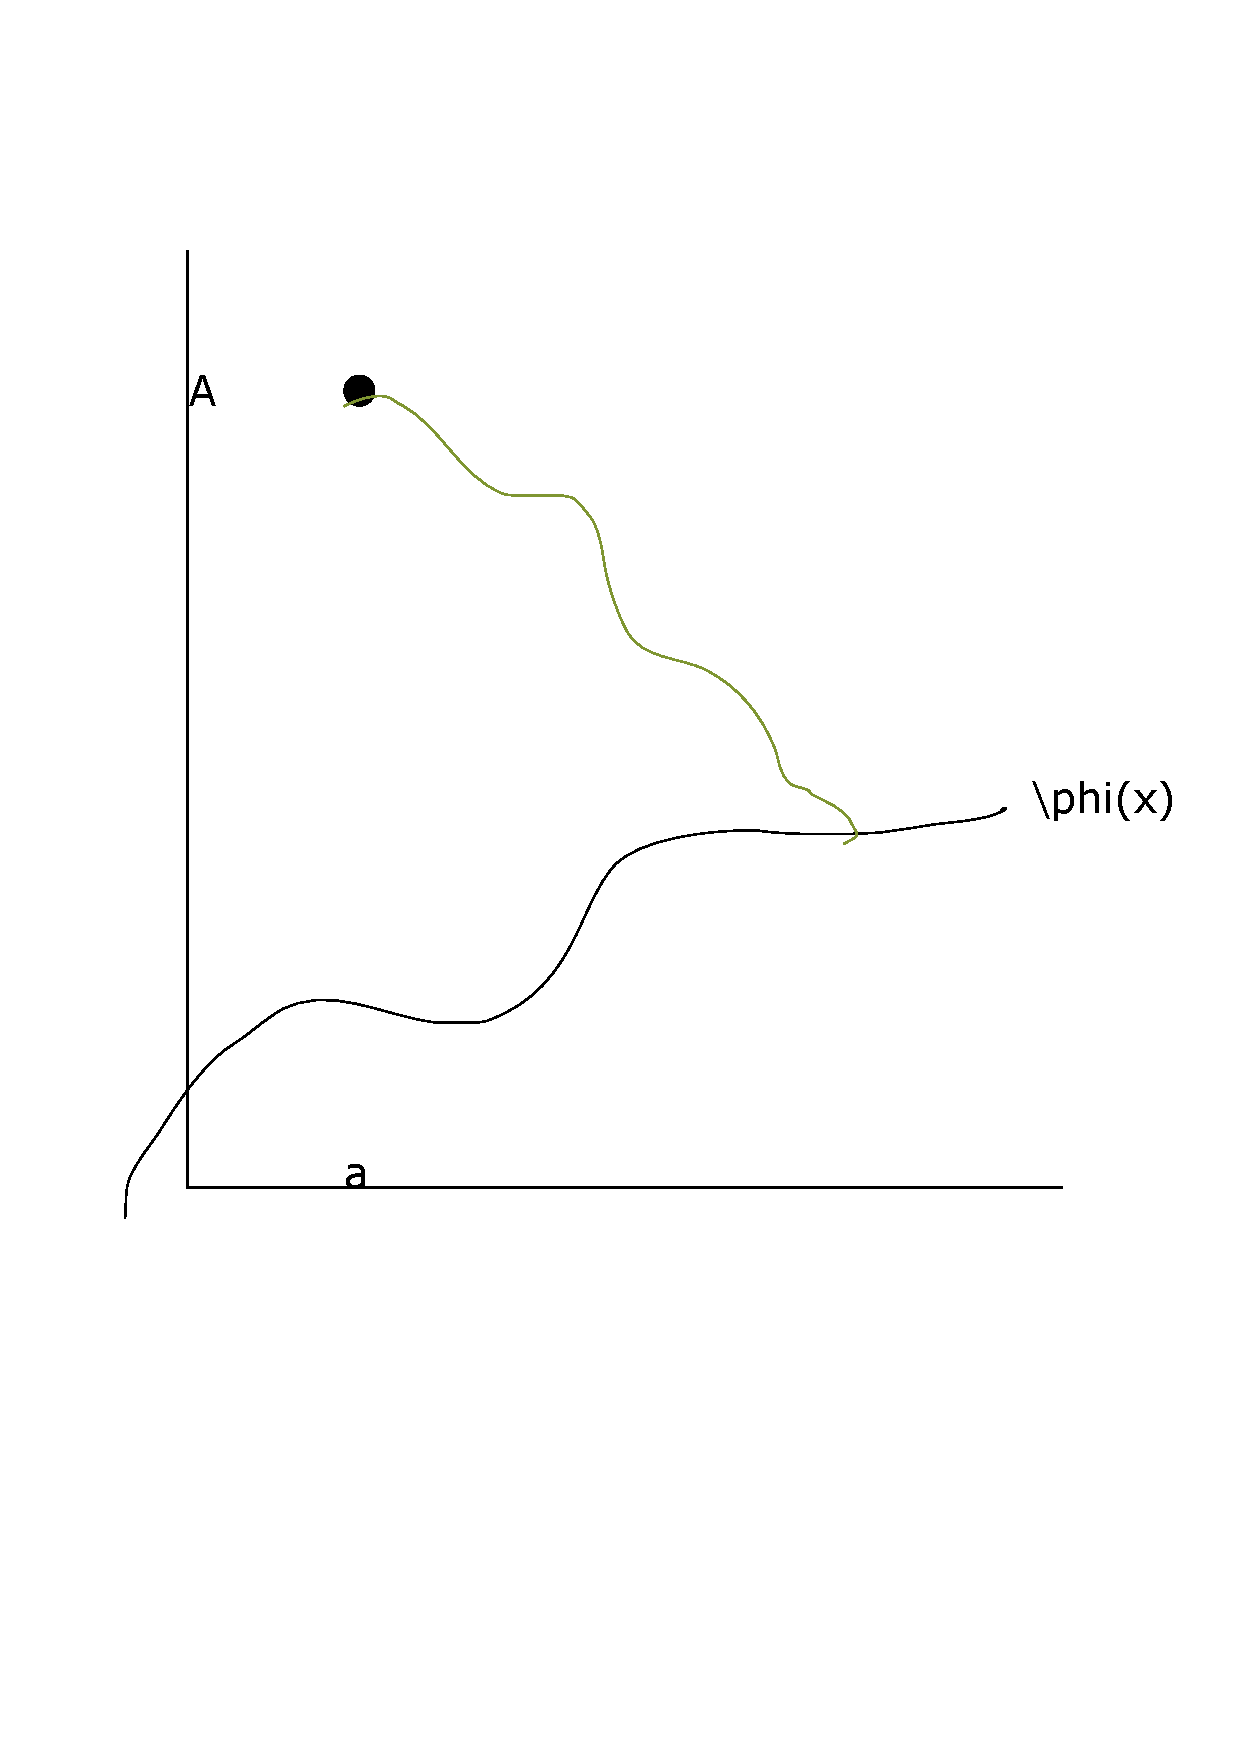
\includegraphics[scale=0.2]{capitolo7.pdf}
\end{flushright}
\end{minipage}
\end{table}

Voglio minimizzare F(u) tra tutte le coppie (u, b) tali che
\[
	u \in C^1([a,b]), u(a)=A, u(b) = \varphi(b)
\]
l'ultima condizione implica che il punto terminale sia sul grafico di $\phi(x)$.
\end{defn}

\begin{oss}
Può essere che b non sia la prima intersezione.
\end{oss}

Vogliamo trovare l'equazione di Eulero-Lagrange in questo caso.

\begin{teo}[Transversality condition]
Se $L \in C^2, \varphi \in C^2$ e $(u_0, x_0) $ minimizza, allora
\[
	[L_p(x, u_0, \dot{u}_0)]'=L_s(x, u_0, \dot{u}_0)\qquad\forall x \in (a, x_0)\text{ : solita ELE}
\]
\[
	u_0(a) = A \text{ : solita DBC}
\]
\[
	L_p(x, u_0(x_0), \dot{u}_0(x_0))[\dot{u}_0(x_0) - \dot{\varphi}(x_0)] = L(x_0, u_0(x_0), \dot{u}_0(x_0))]
\]
L'ultima condizione è detta \textbf{transversality}.
\end{teo}

\begin{oss}
Se $\varphi$ fosse una retta verticale (ma non lo può essere poichè deve essere funzione di x), verrebbe $\dot{\varphi}(x_0) = \infty$ da cui la classica NBC $L_p(x, u_0(x_0), \dot{u}_0(x_0))=0$
\end{oss}

\begin{dimst}
Consideriamo una funzione u(x) ed un punto $x_0$. Consideriamo poi $u + tv$ per una opportuna v(x) che intersecherà $\varphi(x)$. Sia x(t) il punto d'intersezione tra v e $\varphi$.\\
Esistenza ed unicità di x(t) è una questione di teorema delle funzioni implicite, cioè considero 
\[
	\Phi(x, t) := u(x) + tv(x) - \varphi(x)
\]
ed osservo che $\varphi(x_0, 0) = 0$ e spero che per $t \in (-\delta,\delta)$ io possa ricavare x in funzione di t.
\[
	\Phi_t(x, t) = v(x)\quad \Phi_x(x, t) = \dot{u}(x) + t \dot{v}(x) - \dot{\varphi}(x)\ra\Phi_x(x_0, 0) = \dot{u}(x_0) + \dot{\varphi}(x_0)
\]
Se $\dot{u}(x_0) - \dot{\varphi}(x_0) \not = 0$, allora posso ricavare. A questo punto pongo
\[
	\psi(t) := \int_{a}^{x(t)}L(x, u+tv, \dot{u}+t \dot{v})\, dx\ra \psi'(0)=0\footnote{Punto di minimo}.
\]
Quindi
\[
	\psi'(t) = \int_{a}^{x(t)} L_t + L(x(t), u(x(t))+tv(x(t)), \dots) \dot{x}(t)
\]
\[
	\ra \psi'(0) = \int_{a}^{x_0} [L_s(x, u, \dot{u})v + L_p(x, u, \dot{u}) \dot{v}]\, dx + L(x_0, u(x_0), \dots) \dot{x}(0) 
\]
\[
	= \int_{a}^{x_0} [L_s - L_p']v + [L_p(x, u, \dot{u}) \dot{v}]_a^{x_0} + L(x_0, u(x_0), \dots) \dot{x}(0) 
\]
Dal teorema delle funzioni implicite ricavo che 
\[
	\dot{x}(t) = - \frac{\Phi_t(x(t), t)}{\Phi_x(x(t), t)} \leadsto	\dot{x}(0) = -\frac{v(x_0)}{\dot{u}(x_0) - \varphi(x_0)}
\]	
Sostituendo
\[
	\psi'(0) = \int_{a}^{x_0}[L_s - L_p']v + L_p(x_0, u(x_0), \dot{u}(x_0)) \dot{v}(x_0) + L(x_0, u(x_0), \dot{u}(x_0))(-\frac{v(x_0)}{\dot{u}(x_0) - \varphi(x_0)})
\]
Adesso utilizzo funzioni v t.c. $v(x_0)=0$ e da FLCV deduco ELE in (a, $x_0$).\\
Scelgo poi v con $v(x_0)=1$ e ottengo
\[
	L_p(x_0, u(x_0), \dot{u}(x_0)) = \frac{L(x_0, u(x_0), \dot{u}(x_0))}{\dot{u}(x_0) - \dot{\varphi}(x_0) }
\]
Moltiplicando ho la transversality.\\
Passo 2: Supponiamo $\dot{u}(x_0) = \dot{\varphi}(x_0) $.\\
Geometricamente questo significa che l'attacco è "smooth". Uso allora, come competitore, anzichè $u+tv$, la u "allungata".
\[
 	\psi(t) := \int_{a}^{x_0}L(x, u, \dot{u}) + \int_{x_0}^{x_0 + t}L(x, \varphi, \dot{\varphi}) 
 \] 
 \[
 	\psi'(t) = L(x_0 + t, \varphi(x_0 + t), \dot{\vp}(x_0 + t))
 \]
\[
	\ra \psi'(0) = L(x_0, \varphi(x_0), \dot{\vp}(x_0)) = L(x_0, u(x_0), \dot{u}(x_0))
\]

\begin{oss}
Non posso dire che $\psi'(0)=0$ poichè $\psi$ è definita solo per $t \ge 0$.
\end{oss}
Posso dire solo che $\psi'(0)\ge0$ da cui $L(x_0, u(x_0), \dot{u}(x_0))\ge0$.\\
Passo 3: cerco di "accorciare" la u.\\
\textit{inserire immagine minuto 31}\\
In questo caso $\psi(t) = $ funzionale calcolato sulla u accorciata:
\[
	\psi(t) \int_{a}^{x_0 - 2t}L(x, u, \dot{u}) + \int_{x_0-2t}^{x_0-t}L(x, l, \dot{l})
\]
con l: equazione della retta di raccordo
\[
	\ra \psi(t) = \int_{a}^{x_0}L(x, u, \dot{u}) - \int_{x_0-2t}^{x_0}L(x, u, \dot{u}) +  \int_{x_0-2t}^{x_0-t}L(x, l, \dot{l})
\]
Il primo termine è costante, quindi quando derivo sparisce.\\
La derivata del secondo termine è 
\[
	-2L(x_0 - 2t, u(x_0-2t), \dot{u}(x_0-2t))
\]
Perciò quando metto t = 0 ottengo $-2 L(x_0, u(x_0), \dot{u}(x_0)$.\\
Per derivare l'ultimo termine posso scrivere l'equazione di l come retta passante per due punti, oppure osservo che per il teorema della media integrale vale 
\[
	\int_{x_0- 2t}^{x_0-t}L(x, l(x), \dot{l}(x)) = t L(x(t), l(x(t)), \dot{l}(x(t)))
\]
Dividendo per t e passando al limite per $t \to 0$, la derivata del terzo termine è
\[
	L(x_0, u(x_0), \dot{u}(x_0))
\]
poichè $x_0 -2t\le x(t)\le x_0-t$ e $l(x(t)) \in [u(x_0-2t, u(x_0-t))] $. Per passare al limite $\dot{l}(x(t)) \to \dot{u}(x_0)$ serve che $\dot{u}(x_0) = \dot{\varphi}(x_0)$.\\
In conclusione
\[
	\psi'(t) = -L(x_0, u(x_0), \dot{u}(x_0)) \ge 0\quad\text{per }t\ge0
\]
Questo completa la dimostrazione anche nel caso in cui $\dot{u}(x_0) = \dot{\varphi}(x_0)$. \qed
\end{dimst}

\begin{ex}
\[
	F(u, b) = \int_{0}^{b}(\dot{u}^2 + u^2)\, dx
\]
e prendiamo come DBC $u(0) = 1, \varphi(x)\equiv 0 $.\\

\begin{tikzpicture}[scale=1.2]
\draw[->] (-1, 0)  -- (2.5, 0);
\draw[->] (0, -1)  -- (0, 1.5);
\draw (0, 1) node[anchor = north east] {1} .. controls (1/4, 1/6) and (3/2, 1/8) .. (2, 0) node[anchor = south west]{b};
\end{tikzpicture}
Esiste il minimo?\\
ELE: $$L_p' = L_s \ra (2\dot{u})' = 2u \ra \ddot{u} = u \ra u(x) = a cosh(x) + b sinh(x)$$
Da $u(0) = 1$ ottengo che 
\[
	u(x) = cosh(x) + bsinh(x)
\]
Impongo adesso la transversality
\[
	L_p(x, u, \dot{u}) (\dot{u} - \dot{\varphi} ) = L(x, u, \dot{u})\quad\text{in }x_0	
\]
\[
	\ra 2\dot{u}(\dot{u} - 0) = \dot{u}^2 + u^2 \ra \dot{u}^2 = u^2
\]
Nel punto di contatto vale $u(x_0) = 0$, quindi $\dot{u}(x_0)=0$.
\[
 	\ra 
 	\begin{cases}
 	u(x_0) = 0 \\
 	\dot{u}(x_0) = 0
 	\end{cases}
 \] 
 Questo sistema non ha soluzione, in quanto implicherebbe
 \[
 	b = - \frac{sinh(x_0)}{cosh(x_0)} = -\frac{cosh(x_0)}{sinh(x_0)} \ra sinh^2(x_0) = cosh^2(x_0)\to \text{impossibile}
 \]
\end{ex}


\end{document} 